\chapter{Discussion}

\section{Failure cases}

As the algorithm focuses on fitting straight lines, more work is needed to detect curved crop rows (Fig. \ref{fig:cropcurved}). The Hough and RANSAC processes should be adapted to use customs models, not just linear models. This would mean complications when it comes to the detection of vanishing points and thus for outlier elimination.

Another issue is the non-ordered detection of the lines : since the lines are detected by order of prominence, the first line is not necessarily the most centered one. This can be a problem if a large number of lines is present in a picture : a central row may not be part of the main N rows and is only detected when we adjust the number of crop to be detected (as shown in Fig. \ref{fig:missedcrop})
This problem has many solutions : as crops are set in an equidistant way, the distance between two crop rows could be used as an extra constraint. An easier solution would be to perform a search in the middle of two rows when their distance has a high deviation from the average distance between rows in a picture.

Finally, in some extreme cases where bushes are too prominent, the Hough transform detects too many faulty lines and does not manage to calculate a correct vanishing point. The lines kept as "inliers" are the faulty ones.

\begin{figure}[H]
\centering
\begin{subfigure}
    {0.3\textwidth}
    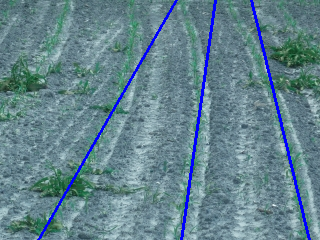
\includegraphics[width=\textwidth]{Report/images/FailureCases/img annotated_ _screenshot_07.01.2023 (2).png}
    \caption{Curved crop rows}
    \label{fig:cropcurved}
\end{subfigure}
\begin{subfigure}{0.3\textwidth}%
    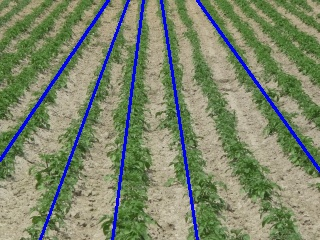
\includegraphics[width=\textwidth]{Report/images/ransaccropskipped.jpg}
    \caption{Wrong order detection}
    \label{fig:missedcrop}

\end{subfigure}
\begin{subfigure}{0.3\textwidth}%
    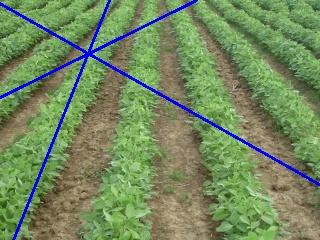
\includegraphics[width=\textwidth]{Report/images/faultyransac.jpg}
    \caption{Bushy crop rows}
    \label{fig:missedcrop}

\end{subfigure}
\end{figure}
\label{pics: bushyremoval}






\section{Future Work}

We have successfully developed an algorithm that detects crop rows in an RGB image or video with high accuracy. Nevertheless, improvements could be made and different cases could be taken into account. 

\begin{enumerate}
    \item Computational time : currently, the algorithm is too slow for real-time applications. A more efficient image processing technique and parallel processing could be implemented. 
    \item Prior information : Our algorithm could be made even more robust by integrating more prior information, such as the distance between crop rows or the number of crop rows
    \item Sensors fusion : integrating
    additional sensors, such as LiDAR, would enhance the algorithm's accuracy
    \item Deep Learning : for even better crop row detection or vegetation segmentation, deep learning could be added
    \item Camera Calibration: The algorithm assumes that the camera is
    calibrated, which means that the intrinsic and extrinsic parameters of
    the camera are known. However, in real-world applications, the camera
    may not be calibrated, or the calibration may drift over time.
    Therefore, it would be beneficial to include an automatic camera
    calibration module to the algorithm to improve its robustness. \\
\end{enumerate}

Of course, the main reason for crop row detection is the navigation of the rover : path planning is another important aspect to consider. This project has concentrated on detecting crop rows and does not provide
information about the optimal path for the robot to follow. This path could be generated using techniques such 
as the A* algorithm, Voronoi diagrams, or other known path planning
techniques to ensure that the robot can navigate efficiently and safely between detected crops. \\

It is also important to note that the dataset used is not representative of all crops: different data sets should be collected to better measure the degree to which the algorithm stays accurate.

